% Created 2015-05-28 Thu 13:42
\documentclass[11pt]{article}
\usepackage[utf8]{inputenc}
\usepackage[T1]{fontenc}
\usepackage{fixltx2e}
\usepackage{graphicx}
\usepackage{longtable}
\usepackage{float}
\usepackage{wrapfig}
\usepackage{rotating}
\usepackage[normalem]{ulem}
\usepackage{amsmath}
\usepackage{textcomp}
\usepackage{marvosym}
\usepackage{wasysym}
\usepackage{amssymb}
\usepackage{capt-of}
\usepackage{hyperref}
\tolerance=1000
\usepackage{minted}
\usepackage{color}
\usepackage{listings}
\usepackage{grffile}
\usepackage[inline]{enumitem}
\usepackage{setspace}
\usepackage{tikz}
\usepackage{subcaption}
\usepackage{xcolor}
\hypersetup{
colorlinks,
linkcolor={red!50!black},
citecolor={blue!50!black},
urlcolor={blue!80!black}
}
\usepackage{setspace}%% The linestretch
\singlespacing
\usepackage[format=hang,indention=0cm,singlelinecheck=true,justification=raggedright,labelfont={normalsize,bf},textfont={normalsize}]{caption} %
\usepackage{vmargin}
\setpapersize{A4}
\setmarginsrb{2.5cm}{1cm}% links, oben
{2.5cm}{2cm}% rechts, unten
{12pt}{30pt}% Kopf: Höhe, Abstand
{12pt}{30pt}% Fuß: Höhe, AB
\usepackage{upquote}
%  use straight quotes when printing a command in minted
\AtBeginDocument{%
\def\PYZsq{\textquotesingle}%
}
\definecolor{mintedbackground}{rgb}{0.95,0.95,0.95}
\setlength{\parindent}{0pt}
\setlength{\parskip}{\baselineskip}
\definecolor{mintedbackground}{rgb}{0.95,0.95,0.95}

%% I detest indentation in footnotes etc, so try this:
\makeatletter
\renewcommand\@makefntext[1]{\noindent\makebox[0em][r]{\@makefnmark}\footnotesize#1}
\makeatother
%% the makeatletter and makeatother are required to allow me to
%% to change the macro beginning with an @. (though when I call it
%% I don't use the @ ... 

\renewcommand\scriptsize\normalsize

\author{Martin Jakt\thanks{University of Nordland, Norway}}
\date{\textbf{Bioinformatics \& Genomics}}
\title{\textbf{Assignment 1 continued} (2015-09-22)}
\hypersetup{
 pdfkeywords={},
  pdfsubject={},
  pdfcreator={}}
\begin{document}

\maketitle
%\tableofcontents

\section{The story so far}
\label{sec-1}
On Monday (21-09-15) you all pretty much managed to take two sequences
and print out a simple dotplot of the two sequences against each other.

For example, for the two sequences \texttt{ATGGGCGA}
and \texttt{ATGCGATT} your scripts printed out something like:
\begin{spacing}{0.75}
\begin{verbatim}
  ATGGGCGA
A *      *
T  *     
G   *** *
C      * 
G   *** * 
A *      *
T  *      
T  *      
\end{verbatim}
\end{spacing}
Where \texttt{*} indicates a match. This lets you visualise potential
alignments between the two sequences by following diagonals from the
top left to the bottom right. However, it doesn't automatically give
you the optimal alignment. For that we need something a bit more complicated.

To turn this into the Needleman-Wunsch dynamic programming algorithm we
need to implement three things:
\begin{enumerate}
\item A two dimensional matrix of alignment scores. This needs an
  extra column, and an extra row to represent initial gaps.
\item A way to store the routes that were followed in obtaining
  the score matrix.
\item A method to extract the alignment from the first two requirements.
\end{enumerate}
The first two of these requirements are rather simple to implement requiring
almost nothing more than we have already covered in the classes. The third
requires the ability to write your own functions, and some understanding of
scope (the parts of your code where a variable can be accessed). Unfortunately,
the most elegant solution to the problem make use of recursion,
where a function calls itself, and this can lead to quite confusing behaviour.

I have written three different scripts, which stepwise implement these
requirements. Scripts 1 and 2, should be reasonably easy to understand,
but the third one implementing the alignment extraction is a little bit
more tricky.

\subsection{A table of alignment scores}
\label{sec-1-1}

\begin{figure}[ht]
  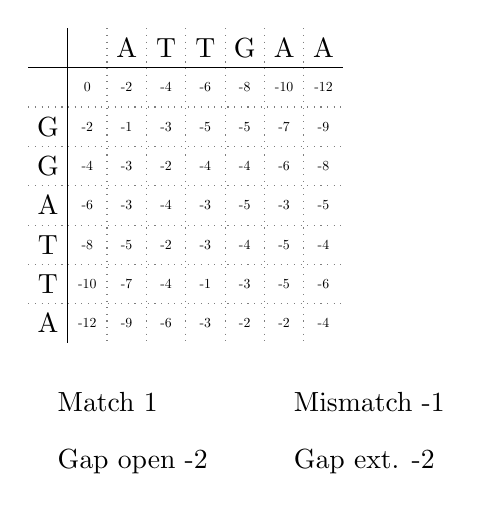
\begin{tikzpicture}[scale=0.5]
    \node [right] at (1,-1) {Match 1};
\node [right] at (7,-1) {Mismatch -1};
\node [right] at (1,-2.5) {Gap open -2};
\node [right] at (7,-2.5) {Gap ext. -2};

\draw [-] (0.5,7.5) -- (8.5,7.5);
\draw [-] (1.5,8.5) -- (1.5,0.5);
\draw [-, dotted, opacity=0.5] (0.5,6.5) -- (8.5,6.5);
\draw [-, dotted, opacity=0.5] (2.5,8.5) -- (2.5,0.5);
	\node at (3,8) {A};
	\draw [-, dotted, opacity=0.5] (3.5,8.5) -- (3.5,0.5);
	\node at (4,8) {T};
	\draw [-, dotted, opacity=0.5] (4.5,8.5) -- (4.5,0.5);
	\node at (5,8) {T};
	\draw [-, dotted, opacity=0.5] (5.5,8.5) -- (5.5,0.5);
	\node at (6,8) {G};
	\draw [-, dotted, opacity=0.5] (6.5,8.5) -- (6.5,0.5);
	\node at (7,8) {A};
	\draw [-, dotted, opacity=0.5] (7.5,8.5) -- (7.5,0.5);
	\node at (8,8) {A};
	\node at (1,6) {G};
	\draw [-, dotted, opacity=0.5] (0.5,5.5) -- (8.5,5.5);
	\node at (1,5) {G};
	\draw [-, dotted, opacity=0.5] (0.5,4.5) -- (8.5,4.5);
	\node at (1,4) {A};
	\draw [-, dotted, opacity=0.5] (0.5,3.5) -- (8.5,3.5);
	\node at (1,3) {T};
	\draw [-, dotted, opacity=0.5] (0.5,2.5) -- (8.5,2.5);
	\node at (1,2) {T};
	\draw [-, dotted, opacity=0.5] (0.5,1.5) -- (8.5,1.5);
	\node at (1,1) {A};

	\node[scale=0.5] at (2,7) {0};
	\node[scale=0.5] at (3,7) {-2};
	%\draw [->] (2.65, 6+1) -- (2.35, 6+1);
	\node[scale=0.5] at(4,7) {-4};
	%\draw [->] (3.65,6+1) -- (3.35,6+1);
	\node[scale=0.5] at(5,7) {-6};
	%\draw [->] (4.65,6+1) -- (4.35,6+1);
	\node[scale=0.5] at(6,7) {-8};
	%\draw [->] (5.65,6+1) -- (5.35,6+1);
	\node[scale=0.5] at(7,7) {-10};
	%\draw [->] (6.65,6+1) -- (6.35,6+1);
	\node[scale=0.5] at(8,7) {-12};
	%\draw [->] (7.65,6+1) -- (7.35,6+1);
	\node[scale=0.5] at (2,6) {-2};
	%\draw [->] (2,6 + 0.35) -- (2, 6 + 0.65);
	\node[scale=0.5] at(2,5) {-4};
	%\draw [->] (2,6-1 + 0.35) -- (2, 6-1 + 0.65);
	\node[scale=0.5] at(2,4) {-6};
	%\draw [->] (2,6-2 + 0.35) -- (2, 6-2 + 0.65);
	\node[scale=0.5] at(2,3) {-8};
	%\draw [->] (2,6-3 + 0.35) -- (2, 6-3 + 0.65);
	\node[scale=0.5] at(2,2) {-10};
	%\draw [->] (2,6-4 + 0.35) -- (2, 6-4 + 0.65);
	\node[scale=0.5] at(2,1) {-12};
	%\draw [->] (2,6-5 + 0.35) -- (2, 6-5 + 0.65);

	\node [scale=0.5] at (3,6) {-1};
	%\draw [->] (2.65,6.35) -- (2.35,6.65);
	\node [scale=0.5] at (4,6) {-3};
	%\draw [->] (3.65,6.35) -- (3.35,6.65);
	%\draw [->] (3.65,6) -- (3.35,6);
	\node [scale=0.5] at (5,6) {-5};
	%\draw [->] (4.65,6.35) -- (4.35,6.65);
	%\draw [->] (4.65,6) -- (4.35,6);
	\node [scale=0.5] at (6,6) {-5};
	%\draw [->] (5.65,6.35) -- (5.35,6.65);
	\node [scale=0.5] at (7,6) {-7};
	%\draw [->] (6.65,6) -- (6.35,6);
	\node [scale=0.5] at (8,6) {-9};
	%\draw [->] (7.65,6) -- (7.35,6);

	\node [scale=0.5] at (3,5) {-3};
	%\draw [->] (2.65,5.35) -- (2.35,5.65);
	%\draw [->] (3,5.35) -- (3,5.65);
	\node [scale=0.5] at (4,5) {-2};
	%\draw [->] (3.65,5.35) -- (3.35,5.65);
	\node [scale=0.5] at (5,5) {-4};
	%\draw [->] (4.65,5.35) -- (4.35,5.65);
	%\draw [->] (4.65,5) -- (4.35,5);
	\node [scale=0.5] at (6,5) {-4};
	%\draw [->] (5.65,5.35) -- (5.35,5.65);
	\node [scale=0.5] at (7,5) {-6};
	%\draw [->] (6.65,5.35) -- (6.35,5.65);
	%\draw [->] (6.65,5) -- (6.35,5);
	\node [scale=0.5] at (8,5) {-8};
	%\draw [->] (7.65,5.35) -- (7.35,5.65);
	%\draw [->] (7.65,5) -- (7.35,5);

	\node [scale=0.5] at (3,4) {-3};
	%\draw [->] (2.65,4.35) -- (2.35,4.65);
	\node [scale=0.5] at (4,4) {-4};
	%\draw [->] (3.65,4.35) -- (3.35,4.65);
	%\draw [->] (4,4.35) -- (4,4.65);
	\node [scale=0.5] at (5,4) {-3};
	%\draw [->] (4.65,4.35) -- (4.35,4.65);
	\node [scale=0.5] at (6,4) {-5};
	%\draw [->] (5.65,4.35) -- (5.35,4.65);
	%\draw [->] (5.65,4) -- (5.35,4);
	\node [scale=0.5] at (7,4) {-3};
	%\draw [->] (6.65,4.35) -- (6.35,4.65);
	\node [scale=0.5] at (8,4) {-5};
	%\draw [->] (7.65,4.35) -- (7.35,4.65);
	%\draw [->] (7.65,4) -- (7.35,4);

	\node [scale=0.5] at (3,3) {-5};
	%\draw [->] (3,3.35) -- (3,3.65);
	\node [scale=0.5] at (4,3) {-2};
	%\draw [->] (3.65,3.35) -- (3.35,3.65);
	\node [scale=0.5] at (5,3) {-3};
	%\draw [->] (4.65,3.35) -- (4.35,3.65);
	\node [scale=0.5] at (6,3) {-4};
	%\draw [->] (5.65,3.35) -- (5.35,3.65);
	\node [scale=0.5] at (7,3) {-5};
	%\draw [->] (7,3.35) -- (7,3.65);
	\node [scale=0.5] at (8,3) {-4};
	%\draw [->] (7.65,3.35) -- (7.35,3.65);

	\node [scale=0.5] at (3,2) {-7};
	%\draw [->] (3,2.35) -- (3,2.65);
	\node [scale=0.5] at (4,2) {-4};
	%\draw [->] (3.65,2.35) -- (3.35,2.65);
	%\draw [->] (4,2.35) -- (4,2.65);
	\node [scale=0.5] at (5,2) {-1};
	%\draw [->] (4.65,2.35) -- (4.35,2.65);
	\node [scale=0.5] at (6,2) {-3};
	%\draw [->] (5.65,2) -- (5.35,2);
	\node [scale=0.5] at (7,2) {-5};
	%\draw [->] (6.65,2.35) -- (6.35,2.65);
	%\draw [->] (6.65,2) -- (6.35,2);
	\node [scale=0.5] at (8,2) {-6};
	%\draw [->] (7.65,2.35) -- (7.35,2.65);
	%\draw [->] (8,2.35) -- (8,2.65);

	\node [scale=0.5] at (3,1) {-9};
	%\draw [->] (2.65,1.35) -- (2.35,1.65);
	%\draw [->] (3,1.35) -- (3,1.65);
	\node [scale=0.5] at (4,1) {-6};
	%\draw [->] (4,1.35) -- (4,1.65);
	\node [scale=0.5] at (5,1) {-3};
	%\draw [->] (5,1.35) -- (5,1.65);
	\node [scale=0.5] at (6,1) {-2};
	%\draw [->] (5.65,1.35) -- (5.35,1.65);
	\node [scale=0.5] at (7,1) {-2};
	%\draw [->] (6.65,1.35) -- (6.35,1.65);
	\node [scale=0.5] at (8,1) {-4};
	%\draw [->] (7.65,1.35) -- (7.35,1.65);
	%\draw [->] (7.65,1) -- (7.35,1);


  \end{tikzpicture}
  \caption{Table of alignment scores. Sequences are shown along the top and
    the side.}
  \label{scoreMatrix}
\end{figure}
Fig. \ref{scoreMatrix} shows a table of alignment scores for a Needleman-Wunsh alignment
where the gap open and extension penalties are the same. 
To 
calculate the scores for two sequences \texttt{as} and \texttt{bs} we first create a two dimensional matrix to hold the
scores. Note that if \texttt{a} has 6 characters then we'll need 7 rows, and
similarly we require 7 columns if \texttt{bs} has 6 characters (as in the example).

As usual we start with the two sequences in two arrays \texttt{@a} and
\texttt{@b}. We then initialise the scoring matrix setting all values to 0:

\begin{minted}[fontsize=\scriptsize,bgcolor=lightgray,linenos]{perl}
for $i(0..@a){        ## $i represents the rows of the table
    for $j(0..@b){    ## $j represents the columns of the table
	$scores[$i][$j] = 0;
    }
}
\end{minted}

Since \texttt{@a} evaluates to the length of the sequence, the range of
values \texttt{0..@a} will have one more entry than the length of \texttt{@a}.

Our next step is to add the initial penalties in the top row and the left most
column. These represent terminal gaps and so we simply add the gap penalties
going from the top left corner:

\begin{minted}[fontsize=\scriptsize,bgcolor=lightgray,linenos]{perl}
## first fill in the top row (which has row number 0).
for $j(1..@b){
    $scores[0][$j] = $scores[0][$j-1] + $gap;
}

## then the first column (has column number 0).
for $i(1..@a){
    $scores[$i][0] = $scores[$i-1][0] + $gap;
}
\end{minted}

For the top row we set the score in column \texttt{j} to be the sum
of the score in column \texttt{j-1} and the gap penalty. We do the same thing
for the rows in the left-most column. The top left position should have a
score of 0, so we do not need to change this. Hence our loop starts from a
value of 1 in both cases.

Now all we need to do is to go through the positions in the matrix (from the
second column and row) and calculate the scores for each position (cell) in
the table. The score at row \texttt{i} and column \texttt{j} should be the max
of:
\begin{enumerate}
\item The mismatch / match score for the corresponding sequence positions +
  the score at \texttt{i-1,j-1} (i.e. diagonally above and to the left). Since
  the second column of the table corresponds to the first position of
  \texttt{as} we have to compare the characters at positions \texttt{i-1} and
  \texttt{j-1}.
\item The gap penalty + the score in the cell immediately to the left (i.e. at
  position \texttt{i, j-1}).
\item The gap penalty + the score in the cell immediately above (i.e. at
  position \texttt{i-1,j}).
\end{enumerate}

\begin{minted}[fontsize=\scriptsize,bgcolor=lightgray,linenos]{perl}
for $i(0..$#a){    
## here $i represents the positions in sequence a.
## hence $i + 1 is equal to the row number of the score
## that we wish to set, and $i itself corresponds to the previous row.
    for $j(0..$#b){
	## similarly, $j corresponds to the previous column, and $j+1
	## to the column of the score that we wish to set.
	
	## first determine these three possible scores. 
        ## We can call the scores $s1, $s2 and $s3 
	## The first of these depends on whether ($a[$i] eq $b[$j])
	
	## this is a bit ugly, but what the hell
	if($a[$i] eq $b[$j]){
	    $s1 = $scores[$i][$j] + $match;
	}else{
	    $s1 = $scores[$i][$j] + $mismatch;
	}
	$s2 = $scores[$i+1][$j] + $gap;
	$s3 = $scores[$i][$j+1] + $gap;

	## now we need to determine which of these is the highest. 
        ## The simplest way of doing this is by something like:
	$max = $s1;
	if($max < $s2){ $max = $s2; }
	if($max < $s3){ $max = $s3; }
	## we don't have to use a new line for conditionals, 
        ## and writing it like this looks a bit neater to me.
	
	## then simply set the score at row ($i + 1) 
        ## and column ($j + 1) to $max.
	$scores[$i+1][$j+1] = $max;
    }
}
\end{minted}

In the above code, the looping variables \texttt{\$i} and \texttt{\$j} refer
to the positions in the sequences, which are one lower than the positions of
the table. Hence we set the value at \texttt{\$scores[\$i+1][\$j+1]}. This is
nice as the diagonally prior cell is \texttt{\$scores[\$i][\$j]}, but can look
a little confusing as it means that the cell to the left is
\texttt{\$scores[\$i+1][\$j]} and the one above is at
\texttt{\$scores[\$i][\$j+1]}.

Now we've completed step 1. However, to be able to look at the results I also
added a small function to make it convenient to print out the
matrix at different stages of the process. This function is defined at the
bottom of the page. It takes no arguments and is called by simply typing:
\begin{minted}[fontsize=\scriptsize,bgcolor=lightgray,linenos]{perl}
print_score_table();
\end{minted}

\begin{minted}[fontsize=\scriptsize,bgcolor=lightgray,linenos]{perl}
## a simple function that prints out the table and the sequences.
## it takes no arguments, but makes use of the global variables
## $scores, @a, @b
sub print_score_table{
    print "\t";
    for $j(0..$#b){
	print "\t", $b[$j];
    }
    print "\n";
    for $i(0..@a){   ## again, $i represents the rows here
	## if $i is 0, then we print a space, otherwise we print
	## $a[$i-1]
	if($i == 0){
	    print "  ";
	}else{
	    print $a[$i-1], " ";
	}
	for $j(0..@b){ ## and $j indicates the rows
	    print "\t", $scores[$i][$j];
	}
	print "\n";
    }
    print "=======================================\n";
}
\end{minted}

In perl you can define functions using the \texttt{sub} keyword. The function
is then defined within the following set of curly brackets (which we call a
block of text or code). Functions can take both arguments (more on that later)
and return values. However, in this case all we want is for the function to
print out some stuff to the screen, so we can make use of global variables
(ones not defined using the \texttt{my} keyword). 

In perl any variables not defined with the
\texttt{my} keyword are accessible (can be read and modified) from anywhere
within the code, including in functions (i.e. they are global). This can be convenient, but can also
be dangerous: for example, in this function I have used the variables
\texttt{\$i} and \texttt{\$j}. If you called \texttt{print\_score\_table()} from
within a loop using \texttt{\$i} or \texttt{\$j} these values would be
modified by the function and you would end up in all sorts of trouble. I
really should have written:

\begin{minted}[fontsize=\scriptsize,bgcolor=lightgray,linenos]{perl}
for my $i(0..@a){
  for my $j(0..@b){
    ## important stuff here
  }
}
\end{minted}

You should not have any trouble understanding the function. Perhaps the only
new thing is the use of \verb|\t|. This indicates a tab stop and can be used
to line up columns of text (albeit rather uglily).


\begin{figure}[ht]
\begin{verbatim}
                A       T       T       G       A       A                                                                                                                                            
        0       -2      -4      -6      -8      -10     -12                                                                                                                                          
G       -2      -1      -3      -5      -5      -7      -9                                                                                                                                           
G       -4      -3      -2      -4      -4      -6      -8                                                                                                                                           
A       -6      -3      -4      -3      -5      -3      -5                                                                                                                                           
T       -8      -5      -2      -3      -4      -5      -4                                                                                                                                           
T       -10     -7      -4      -1      -3      -5      -6                                                                                                                                           
A       -12     -9      -6      -3      -2      -2      -4                                                                                                                                           
=======================================  
\end{verbatim}
\caption{Table of alignment scores printed out by needleman\_wunsch\_step1.pl}
\label{s1Table}
\end{figure}
The final output of this when running the script with the sequences 
shown in Fig. \ref{scoreMatrix} are displayed in Fig. \ref{s1Table}.
Somewhat pleasingly these values correspond to the values in Fig. \ref{scoreMatrix} which I
obtained by running a different script that can be used to plot the values in
using Latex. That script has quite a different structure, so getting the same
values suggest that something is correct.

\subsection{Remembering the route}
\label{sec-1-2}
\begin{figure}[ht]
  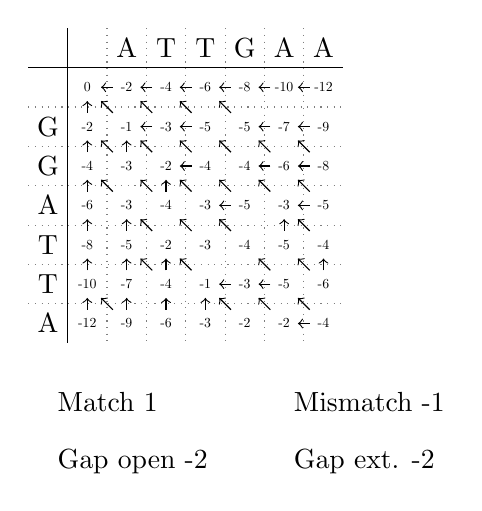
\begin{tikzpicture}[scale=0.5]
    \node [right] at (1,-1) {Match 1};
\node [right] at (7,-1) {Mismatch -1};
\node [right] at (1,-2.5) {Gap open -2};
\node [right] at (7,-2.5) {Gap ext. -2};

\draw [-] (0.5,7.5) -- (8.5,7.5);
\draw [-] (1.5,8.5) -- (1.5,0.5);
\draw [-, dotted, opacity=0.5] (0.5,6.5) -- (8.5,6.5);
\draw [-, dotted, opacity=0.5] (2.5,8.5) -- (2.5,0.5);
	\node at (3,8) {A};
	\draw [-, dotted, opacity=0.5] (3.5,8.5) -- (3.5,0.5);
	\node at (4,8) {T};
	\draw [-, dotted, opacity=0.5] (4.5,8.5) -- (4.5,0.5);
	\node at (5,8) {T};
	\draw [-, dotted, opacity=0.5] (5.5,8.5) -- (5.5,0.5);
	\node at (6,8) {G};
	\draw [-, dotted, opacity=0.5] (6.5,8.5) -- (6.5,0.5);
	\node at (7,8) {A};
	\draw [-, dotted, opacity=0.5] (7.5,8.5) -- (7.5,0.5);
	\node at (8,8) {A};
	\node at (1,6) {G};
	\draw [-, dotted, opacity=0.5] (0.5,5.5) -- (8.5,5.5);
	\node at (1,5) {G};
	\draw [-, dotted, opacity=0.5] (0.5,4.5) -- (8.5,4.5);
	\node at (1,4) {A};
	\draw [-, dotted, opacity=0.5] (0.5,3.5) -- (8.5,3.5);
	\node at (1,3) {T};
	\draw [-, dotted, opacity=0.5] (0.5,2.5) -- (8.5,2.5);
	\node at (1,2) {T};
	\draw [-, dotted, opacity=0.5] (0.5,1.5) -- (8.5,1.5);
	\node at (1,1) {A};

	\node[scale=0.5] at (2,7) {0};
	\node[scale=0.5] at (3,7) {-2};
	\draw [->] (2.65, 6+1) -- (2.35, 6+1);
	\node[scale=0.5] at(4,7) {-4};
	\draw [->] (3.65,6+1) -- (3.35,6+1);
	\node[scale=0.5] at(5,7) {-6};
	\draw [->] (4.65,6+1) -- (4.35,6+1);
	\node[scale=0.5] at(6,7) {-8};
	\draw [->] (5.65,6+1) -- (5.35,6+1);
	\node[scale=0.5] at(7,7) {-10};
	\draw [->] (6.65,6+1) -- (6.35,6+1);
	\node[scale=0.5] at(8,7) {-12};
	\draw [->] (7.65,6+1) -- (7.35,6+1);
	\node[scale=0.5] at (2,6) {-2};
	\draw [->] (2,6 + 0.35) -- (2, 6 + 0.65);
	\node[scale=0.5] at(2,5) {-4};
	\draw [->] (2,6-1 + 0.35) -- (2, 6-1 + 0.65);
	\node[scale=0.5] at(2,4) {-6};
	\draw [->] (2,6-2 + 0.35) -- (2, 6-2 + 0.65);
	\node[scale=0.5] at(2,3) {-8};
	\draw [->] (2,6-3 + 0.35) -- (2, 6-3 + 0.65);
	\node[scale=0.5] at(2,2) {-10};
	\draw [->] (2,6-4 + 0.35) -- (2, 6-4 + 0.65);
	\node[scale=0.5] at(2,1) {-12};
	\draw [->] (2,6-5 + 0.35) -- (2, 6-5 + 0.65);

	\node [scale=0.5] at (3,6) {-1};
	\draw [->] (2.65,6.35) -- (2.35,6.65);
	\node [scale=0.5] at (4,6) {-3};
	\draw [->] (3.65,6.35) -- (3.35,6.65);
	\draw [->] (3.65,6) -- (3.35,6);
	\node [scale=0.5] at (5,6) {-5};
	\draw [->] (4.65,6.35) -- (4.35,6.65);
	\draw [->] (4.65,6) -- (4.35,6);
	\node [scale=0.5] at (6,6) {-5};
	\draw [->] (5.65,6.35) -- (5.35,6.65);
	\node [scale=0.5] at (7,6) {-7};
	\draw [->] (6.65,6) -- (6.35,6);
	\node [scale=0.5] at (8,6) {-9};
	\draw [->] (7.65,6) -- (7.35,6);

	\node [scale=0.5] at (3,5) {-3};
	\draw [->] (2.65,5.35) -- (2.35,5.65);
	\draw [->] (3,5.35) -- (3,5.65);
	\node [scale=0.5] at (4,5) {-2};
	\draw [->] (3.65,5.35) -- (3.35,5.65);
	\node [scale=0.5] at (5,5) {-4};
	\draw [->] (4.65,5.35) -- (4.35,5.65);
	\draw [->] (4.65,5) -- (4.35,5);
	\node [scale=0.5] at (6,5) {-4};
	\draw [->] (5.65,5.35) -- (5.35,5.65);
	\node [scale=0.5] at (7,5) {-6};
	\draw [->] (6.65,5.35) -- (6.35,5.65);
	\draw [->] (6.65,5) -- (6.35,5);
	\node [scale=0.5] at (8,5) {-8};
	\draw [->] (7.65,5.35) -- (7.35,5.65);
	\draw [->] (7.65,5) -- (7.35,5);

	\node [scale=0.5] at (3,4) {-3};
	\draw [->] (2.65,4.35) -- (2.35,4.65);
	\node [scale=0.5] at (4,4) {-4};
	\draw [->] (3.65,4.35) -- (3.35,4.65);
	\draw [->] (4,4.35) -- (4,4.65);
	\node [scale=0.5] at (5,4) {-3};
	\draw [->] (4.65,4.35) -- (4.35,4.65);
	\node [scale=0.5] at (6,4) {-5};
	\draw [->] (5.65,4.35) -- (5.35,4.65);
	\draw [->] (5.65,4) -- (5.35,4);
	\node [scale=0.5] at (7,4) {-3};
	\draw [->] (6.65,4.35) -- (6.35,4.65);
	\node [scale=0.5] at (8,4) {-5};
	\draw [->] (7.65,4.35) -- (7.35,4.65);
	\draw [->] (7.65,4) -- (7.35,4);

	\node [scale=0.5] at (3,3) {-5};
	\draw [->] (3,3.35) -- (3,3.65);
	\node [scale=0.5] at (4,3) {-2};
	\draw [->] (3.65,3.35) -- (3.35,3.65);
	\node [scale=0.5] at (5,3) {-3};
	\draw [->] (4.65,3.35) -- (4.35,3.65);
	\node [scale=0.5] at (6,3) {-4};
	\draw [->] (5.65,3.35) -- (5.35,3.65);
	\node [scale=0.5] at (7,3) {-5};
	\draw [->] (7,3.35) -- (7,3.65);
	\node [scale=0.5] at (8,3) {-4};
	\draw [->] (7.65,3.35) -- (7.35,3.65);

	\node [scale=0.5] at (3,2) {-7};
	\draw [->] (3,2.35) -- (3,2.65);
	\node [scale=0.5] at (4,2) {-4};
	\draw [->] (3.65,2.35) -- (3.35,2.65);
	\draw [->] (4,2.35) -- (4,2.65);
	\node [scale=0.5] at (5,2) {-1};
	\draw [->] (4.65,2.35) -- (4.35,2.65);
	\node [scale=0.5] at (6,2) {-3};
	\draw [->] (5.65,2) -- (5.35,2);
	\node [scale=0.5] at (7,2) {-5};
	\draw [->] (6.65,2.35) -- (6.35,2.65);
	\draw [->] (6.65,2) -- (6.35,2);
	\node [scale=0.5] at (8,2) {-6};
	\draw [->] (7.65,2.35) -- (7.35,2.65);
	\draw [->] (8,2.35) -- (8,2.65);

	\node [scale=0.5] at (3,1) {-9};
	\draw [->] (2.65,1.35) -- (2.35,1.65);
	\draw [->] (3,1.35) -- (3,1.65);
	\node [scale=0.5] at (4,1) {-6};
	\draw [->] (4,1.35) -- (4,1.65);
	\node [scale=0.5] at (5,1) {-3};
	\draw [->] (5,1.35) -- (5,1.65);
	\node [scale=0.5] at (6,1) {-2};
	\draw [->] (5.65,1.35) -- (5.35,1.65);
	\node [scale=0.5] at (7,1) {-2};
	\draw [->] (6.65,1.35) -- (6.35,1.65);
	\node [scale=0.5] at (8,1) {-4};
	\draw [->] (7.65,1.35) -- (7.35,1.65);
	\draw [->] (7.65,1) -- (7.35,1);


  \end{tikzpicture}
  \caption{Table of alignment scores, with arrows indicating the route of the
    scores. Sequences are shown along the top and
    the side.}
  \label{routeMatrix}
\end{figure}

When we calculated the alignment scores for the table we found the maximal of
three values which depended on values determined at earlier steps and
representing earlier positions in potential alignments. To be able to derive
the alignment we need to remember which positions in the table (matrix)
were used when obtaining the maximal value. These relationships are shown in
Fig. \ref{routeMatrix} as arrows. However in perl we can't use arrows as we don't have a
convenient way to represent them\footnote{This isn't completely true; in more
  low level languages these are a very nice fit for pointers, and even in perl
  we have something similar called references. However the perl syntax for references is
  fairly horrible so I've stayed away from those here.}.

There are lots of ways in which we can represent which cells were used to
calculate the values for a given cell. Since we know that the value must come
from one or more of three positions we can give each of those positions a
carefully chosen value and take the sum of those values to indicate the route
used. If we chose values that are exact powers of two (1, 2, 4, 8, ...) then
any sum is guaranteed to uniquely encode a specific combination of
values. This is essentially a bitwise mask, and will be explained later.

Hence in this case to encode the relationships of the cells used I created an
additional matrix (i.e. table) containing the sum of a combination of 1, 2, or
4 where 1 indicates a diagonal movement, and 2 and 4 indicate horizontal and
vertical movements respectively. I called this matrix (same as a two-dimensional array, or
a table, etc...) \texttt{@routes} and modified the code to first initialise it
to 0:

\begin{minted}[fontsize=\scriptsize,bgcolor=lightgray,linenos]{perl}
for $i(0..@a){        ## $i represents the rows of the table
    for $j(0..@b){    ## $j represents the columns of the table
	$scores[$i][$j] = 0;
	$routes[$i][$j] = 0;
    }
}
\end{minted}

And then to when calculating the values we can also set this depending on
which values we use. This was done simply by adding the following to the
previous code:

\begin{minted}[fontsize=\scriptsize,bgcolor=lightgray,linenos]{perl}
        ## $s1, $s2 and $s3 are the scores for the diagonal, horizontal
        ## and vertically prior cells calculated previously in the code.
	if($s1 == $max){ $routes[$i+1][$j+1] += 1; }
	if($s2 == $max){ $routes[$i+1][$j+1] += 2; }
	if($s3 == $max){ $routes[$i+1][$j+1] += 4; } 
\end{minted}

Remember that \texttt{\$s1}, \texttt{\$s2}, and \texttt{\$s3} are the scores
obtained from the diagonally, horizontally or vertically prior cell (see the code above), and that
\texttt{\$max} contains the maximal value. This is not very pretty, but it
works and it's simple.

I also modified the \verb|print_score_table()| function to make use of an
argument so that it can be used to print out either the score or the route table. 

In perl, arguments are passed to functions as an array which can
be accessed within the function using as \verb|@_|. So all I had to do was
modify the function to print out values from \verb|@_| rather than from
the global variable \texttt{@scores} as was done in the first step. To make it
more readable I actually did:

\begin{minted}[fontsize=\scriptsize,bgcolor=lightgray,linenos]{perl}
sub print_score_table{
  my @table = @_; ## arguments are passed to functions in the @_ array;
## and then used @table that to print the values
\end{minted}

To use this in the code we simply write \verb|print_score_table(@scores)| or 
\verb|print_score_table(@routes)| depending on what we wish to do.
This finally gives us the following for the same sequences used in Fig. \ref{routeMatrix}.
\pagebreak

\begin{figure}[ht]
\begin{verbatim}
                A       T       T       G       A       A
        0       0       0       0       0       0       0
G       0       1       3       3       1       2       2
G       0       5       1       3       1       3       3
A       0       1       5       1       3       1       3
T       0       4       1       1       1       4       1
T       0       4       5       1       2       3       5
A       0       5       4       4       1       1       3
=======================================
\end{verbatim}
\caption{The routing matrix obtained by \texttt{needleman\_wunsch\_step2.pl}. 
  The numbers indicate from which prior cell the maximal score was obtained.
  1) diagonally prior only, 2) horizontally prior only, 4) vertically prior only,
  other numbers indicate combinations of prior cells. Compare these values to
  the arrows in Fig. \ref{routeMatrix}.}
% \caption{hello \texttt{needleman\_wunsch\_step2.pl} }
\label{s2Table}
\end{figure}

Here 1 indicates the score was obtained from the diagonally prior only, 3
diagonally and horizontally prior cells, 5 diagonally and vertically prior cells.
2 and 4 indicate derivation from only horizontal or vertical priors.
6 would indicate both horizontal and vertical movements, but we don't get
that, and neither do we get 7 indicating that we got the same score from all
three alternatives. Note that the values correspond to the arrows in Fig. \ref{routeMatrix}
so the script seems to work!  

\subsection{Extracting the alignment}
\label{sec-1-3}
\begin{figure}[ht]
  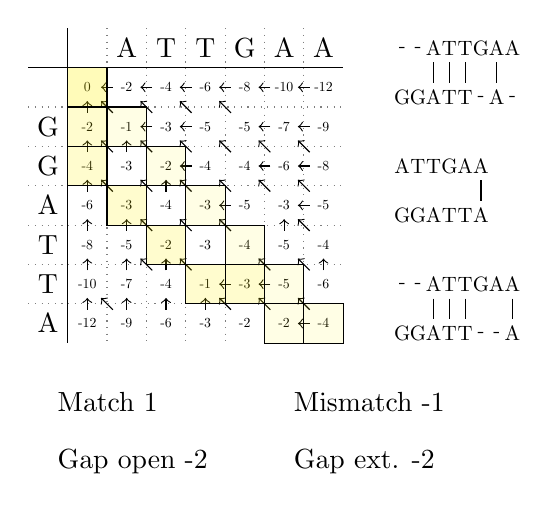
\begin{tikzpicture}[scale=0.5]
    \node [right] at (1,-1) {Match 1};
\node [right] at (7,-1) {Mismatch -1};
\node [right] at (1,-2.5) {Gap open -2};
\node [right] at (7,-2.5) {Gap ext. -2};

\draw [-] (0.5,7.5) -- (8.5,7.5);
\draw [-] (1.5,8.5) -- (1.5,0.5);
\draw [-, dotted, opacity=0.5] (0.5,6.5) -- (8.5,6.5);
\draw [-, dotted, opacity=0.5] (2.5,8.5) -- (2.5,0.5);
	\node at (3,8) {A};
	\draw [-, dotted, opacity=0.5] (3.5,8.5) -- (3.5,0.5);
	\node at (4,8) {T};
	\draw [-, dotted, opacity=0.5] (4.5,8.5) -- (4.5,0.5);
	\node at (5,8) {T};
	\draw [-, dotted, opacity=0.5] (5.5,8.5) -- (5.5,0.5);
	\node at (6,8) {G};
	\draw [-, dotted, opacity=0.5] (6.5,8.5) -- (6.5,0.5);
	\node at (7,8) {A};
	\draw [-, dotted, opacity=0.5] (7.5,8.5) -- (7.5,0.5);
	\node at (8,8) {A};
	\node at (1,6) {G};
	\draw [-, dotted, opacity=0.5] (0.5,5.5) -- (8.5,5.5);
	\node at (1,5) {G};
	\draw [-, dotted, opacity=0.5] (0.5,4.5) -- (8.5,4.5);
	\node at (1,4) {A};
	\draw [-, dotted, opacity=0.5] (0.5,3.5) -- (8.5,3.5);
	\node at (1,3) {T};
	\draw [-, dotted, opacity=0.5] (0.5,2.5) -- (8.5,2.5);
	\node at (1,2) {T};
	\draw [-, dotted, opacity=0.5] (0.5,1.5) -- (8.5,1.5);
	\node at (1,1) {A};

	\node[scale=0.5] at (2,7) {0};
	\node[scale=0.5] at (3,7) {-2};
	\draw [->] (2.65, 6+1) -- (2.35, 6+1);
	\node[scale=0.5] at(4,7) {-4};
	\draw [->] (3.65,6+1) -- (3.35,6+1);
	\node[scale=0.5] at(5,7) {-6};
	\draw [->] (4.65,6+1) -- (4.35,6+1);
	\node[scale=0.5] at(6,7) {-8};
	\draw [->] (5.65,6+1) -- (5.35,6+1);
	\node[scale=0.5] at(7,7) {-10};
	\draw [->] (6.65,6+1) -- (6.35,6+1);
	\node[scale=0.5] at(8,7) {-12};
	\draw [->] (7.65,6+1) -- (7.35,6+1);
	\node[scale=0.5] at (2,6) {-2};
	\draw [->] (2,6 + 0.35) -- (2, 6 + 0.65);
	\node[scale=0.5] at(2,5) {-4};
	\draw [->] (2,6-1 + 0.35) -- (2, 6-1 + 0.65);
	\node[scale=0.5] at(2,4) {-6};
	\draw [->] (2,6-2 + 0.35) -- (2, 6-2 + 0.65);
	\node[scale=0.5] at(2,3) {-8};
	\draw [->] (2,6-3 + 0.35) -- (2, 6-3 + 0.65);
	\node[scale=0.5] at(2,2) {-10};
	\draw [->] (2,6-4 + 0.35) -- (2, 6-4 + 0.65);
	\node[scale=0.5] at(2,1) {-12};
	\draw [->] (2,6-5 + 0.35) -- (2, 6-5 + 0.65);

	\node [scale=0.5] at (3,6) {-1};
	\draw [->] (2.65,6.35) -- (2.35,6.65);
	\node [scale=0.5] at (4,6) {-3};
	\draw [->] (3.65,6.35) -- (3.35,6.65);
	\draw [->] (3.65,6) -- (3.35,6);
	\node [scale=0.5] at (5,6) {-5};
	\draw [->] (4.65,6.35) -- (4.35,6.65);
	\draw [->] (4.65,6) -- (4.35,6);
	\node [scale=0.5] at (6,6) {-5};
	\draw [->] (5.65,6.35) -- (5.35,6.65);
	\node [scale=0.5] at (7,6) {-7};
	\draw [->] (6.65,6) -- (6.35,6);
	\node [scale=0.5] at (8,6) {-9};
	\draw [->] (7.65,6) -- (7.35,6);

	\node [scale=0.5] at (3,5) {-3};
	\draw [->] (2.65,5.35) -- (2.35,5.65);
	\draw [->] (3,5.35) -- (3,5.65);
	\node [scale=0.5] at (4,5) {-2};
	\draw [->] (3.65,5.35) -- (3.35,5.65);
	\node [scale=0.5] at (5,5) {-4};
	\draw [->] (4.65,5.35) -- (4.35,5.65);
	\draw [->] (4.65,5) -- (4.35,5);
	\node [scale=0.5] at (6,5) {-4};
	\draw [->] (5.65,5.35) -- (5.35,5.65);
	\node [scale=0.5] at (7,5) {-6};
	\draw [->] (6.65,5.35) -- (6.35,5.65);
	\draw [->] (6.65,5) -- (6.35,5);
	\node [scale=0.5] at (8,5) {-8};
	\draw [->] (7.65,5.35) -- (7.35,5.65);
	\draw [->] (7.65,5) -- (7.35,5);

	\node [scale=0.5] at (3,4) {-3};
	\draw [->] (2.65,4.35) -- (2.35,4.65);
	\node [scale=0.5] at (4,4) {-4};
	\draw [->] (3.65,4.35) -- (3.35,4.65);
	\draw [->] (4,4.35) -- (4,4.65);
	\node [scale=0.5] at (5,4) {-3};
	\draw [->] (4.65,4.35) -- (4.35,4.65);
	\node [scale=0.5] at (6,4) {-5};
	\draw [->] (5.65,4.35) -- (5.35,4.65);
	\draw [->] (5.65,4) -- (5.35,4);
	\node [scale=0.5] at (7,4) {-3};
	\draw [->] (6.65,4.35) -- (6.35,4.65);
	\node [scale=0.5] at (8,4) {-5};
	\draw [->] (7.65,4.35) -- (7.35,4.65);
	\draw [->] (7.65,4) -- (7.35,4);

	\node [scale=0.5] at (3,3) {-5};
	\draw [->] (3,3.35) -- (3,3.65);
	\node [scale=0.5] at (4,3) {-2};
	\draw [->] (3.65,3.35) -- (3.35,3.65);
	\node [scale=0.5] at (5,3) {-3};
	\draw [->] (4.65,3.35) -- (4.35,3.65);
	\node [scale=0.5] at (6,3) {-4};
	\draw [->] (5.65,3.35) -- (5.35,3.65);
	\node [scale=0.5] at (7,3) {-5};
	\draw [->] (7,3.35) -- (7,3.65);
	\node [scale=0.5] at (8,3) {-4};
	\draw [->] (7.65,3.35) -- (7.35,3.65);

	\node [scale=0.5] at (3,2) {-7};
	\draw [->] (3,2.35) -- (3,2.65);
	\node [scale=0.5] at (4,2) {-4};
	\draw [->] (3.65,2.35) -- (3.35,2.65);
	\draw [->] (4,2.35) -- (4,2.65);
	\node [scale=0.5] at (5,2) {-1};
	\draw [->] (4.65,2.35) -- (4.35,2.65);
	\node [scale=0.5] at (6,2) {-3};
	\draw [->] (5.65,2) -- (5.35,2);
	\node [scale=0.5] at (7,2) {-5};
	\draw [->] (6.65,2.35) -- (6.35,2.65);
	\draw [->] (6.65,2) -- (6.35,2);
	\node [scale=0.5] at (8,2) {-6};
	\draw [->] (7.65,2.35) -- (7.35,2.65);
	\draw [->] (8,2.35) -- (8,2.65);

	\node [scale=0.5] at (3,1) {-9};
	\draw [->] (2.65,1.35) -- (2.35,1.65);
	\draw [->] (3,1.35) -- (3,1.65);
	\node [scale=0.5] at (4,1) {-6};
	\draw [->] (4,1.35) -- (4,1.65);
	\node [scale=0.5] at (5,1) {-3};
	\draw [->] (5,1.35) -- (5,1.65);
	\node [scale=0.5] at (6,1) {-2};
	\draw [->] (5.65,1.35) -- (5.35,1.65);
	\node [scale=0.5] at (7,1) {-2};
	\draw [->] (6.65,1.35) -- (6.35,1.65);
	\node [scale=0.5] at (8,1) {-4};
	\draw [->] (7.65,1.35) -- (7.35,1.65);
	\draw [->] (7.65,1) -- (7.35,1);

\draw [fill=yellow, fill opacity=0.1] (7.5,0.5) rectangle (8.5,1.5);


\draw [fill=yellow, fill opacity=0.1] (6.5,1.5) rectangle (7.5,2.5);


\draw [fill=yellow, fill opacity=0.1] (5.5,2.5) rectangle (6.5,3.5);


\draw [fill=yellow, fill opacity=0.1] (4.5,3.5) rectangle (5.5,4.5);


\draw [fill=yellow, fill opacity=0.1] (3.5,4.5) rectangle (4.5,5.5);


\draw [fill=yellow, fill opacity=0.1] (2.5,5.5) rectangle (3.5,6.5);


\draw [fill=yellow, fill opacity=0.1] (1.5,6.5) rectangle (2.5,7.5);


\draw [fill=yellow, fill opacity=0.1] (5.5,1.5) rectangle (6.5,2.5);


\draw [fill=yellow, fill opacity=0.1] (4.5,1.5) rectangle (5.5,2.5);


\draw [fill=yellow, fill opacity=0.1] (3.5,2.5) rectangle (4.5,3.5);


\draw [fill=yellow, fill opacity=0.1] (2.5,3.5) rectangle (3.5,4.5);


\draw [fill=yellow, fill opacity=0.1] (1.5,4.5) rectangle (2.5,5.5);


\draw [fill=yellow, fill opacity=0.1] (1.5,5.5) rectangle (2.5,6.5);


\draw [fill=yellow, fill opacity=0.1] (1.5,6.5) rectangle (2.5,7.5);


\draw [fill=yellow, fill opacity=0.1] (6.5,0.5) rectangle (7.5,1.5);


\draw [fill=yellow, fill opacity=0.1] (5.5,1.5) rectangle (6.5,2.5);


\draw [fill=yellow, fill opacity=0.1] (4.5,1.5) rectangle (5.5,2.5);

\draw [fill=yellow, fill opacity=0.1] (3.5,2.5) rectangle (4.5,3.5);

\draw [fill=yellow, fill opacity=0.1] (2.5,3.5) rectangle (3.5,4.5);

\draw [fill=yellow, fill opacity=0.1] (1.5,4.5) rectangle (2.5,5.5);

\draw [fill=yellow, fill opacity=0.1] (1.5,5.5) rectangle (2.5,6.5);

\draw [fill=yellow, fill opacity=0.1] (1.5,6.5) rectangle (2.5,7.5);


\node [scale=0.75] (s1) at (10 + 0/2.5, 5) {A};
\node [scale=0.75] (s2) at (10 + 0/2.5, 5-1.25) {G};
\node [scale=0.75] (s1) at (10 + 1/2.5, 5) {T};
\node [scale=0.75] (s2) at (10 + 1/2.5, 5-1.25) {G};
\node [scale=0.75] (s1) at (10 + 2/2.5, 5) {T};
\node [scale=0.75] (s2) at (10 + 2/2.5, 5-1.25) {A};
\node [scale=0.75] (s1) at (10 + 3/2.5, 5) {G};
\node [scale=0.75] (s2) at (10 + 3/2.5, 5-1.25) {T};
\node [scale=0.75] (s1) at (10 + 4/2.5, 5) {A};
\node [scale=0.75] (s2) at (10 + 4/2.5, 5-1.25) {T};
\node [scale=0.75] (s1) at (10 + 5/2.5, 5) {A};
\node [scale=0.75] (s2) at (10 + 5/2.5, 5-1.25) {A};
\draw [-] (s1) -- (s2);
\node [scale=0.75] (s1) at (10 + 0/2.5, 2) {-};
\node [scale=0.75] (s2) at (10 + 0/2.5, 2-1.25) {G};
\node [scale=0.75] (s1) at (10 + 1/2.5, 2) {-};
\node [scale=0.75] (s2) at (10 + 1/2.5, 2-1.25) {G};
\node [scale=0.75] (s1) at (10 + 2/2.5, 2) {A};
\node [scale=0.75] (s2) at (10 + 2/2.5, 2-1.25) {A};
\draw [-] (s1) -- (s2);
\node [scale=0.75] (s1) at (10 + 3/2.5, 2) {T};
\node [scale=0.75] (s2) at (10 + 3/2.5, 2-1.25) {T};
\draw [-] (s1) -- (s2);
\node [scale=0.75] (s1) at (10 + 4/2.5, 2) {T};
\node [scale=0.75] (s2) at (10 + 4/2.5, 2-1.25) {T};
\draw [-] (s1) -- (s2);
\node [scale=0.75] (s1) at (10 + 5/2.5, 2) {G};
\node [scale=0.75] (s2) at (10 + 5/2.5, 2-1.25) {-};
\node [scale=0.75] (s1) at (10 + 6/2.5, 2) {A};
\node [scale=0.75] (s2) at (10 + 6/2.5, 2-1.25) {-};
\node [scale=0.75] (s1) at (10 + 7/2.5, 2) {A};
\node [scale=0.75] (s2) at (10 + 7/2.5, 2-1.25) {A};
\draw [-] (s1) -- (s2);
\node [scale=0.75] (s1) at (10 + 0/2.5, 8) {-};
\node [scale=0.75] (s2) at (10 + 0/2.5, 8-1.25) {G};
\node [scale=0.75] (s1) at (10 + 1/2.5, 8) {-};
\node [scale=0.75] (s2) at (10 + 1/2.5, 8-1.25) {G};
\node [scale=0.75] (s1) at (10 + 2/2.5, 8) {A};
\node [scale=0.75] (s2) at (10 + 2/2.5, 8-1.25) {A};
\draw [-] (s1) -- (s2);
\node [scale=0.75] (s1) at (10 + 3/2.5, 8) {T};
\node [scale=0.75] (s2) at (10 + 3/2.5, 8-1.25) {T};
\draw [-] (s1) -- (s2);
\node [scale=0.75] (s1) at (10 + 4/2.5, 8) {T};
\node [scale=0.75] (s2) at (10 + 4/2.5, 8-1.25) {T};
\draw [-] (s1) -- (s2);
\node [scale=0.75] (s1) at (10 + 5/2.5, 8) {G};
\node [scale=0.75] (s2) at (10 + 5/2.5, 8-1.25) {-};
\node [scale=0.75] (s1) at (10 + 6/2.5, 8) {A};
\node [scale=0.75] (s2) at (10 + 6/2.5, 8-1.25) {A};
\draw [-] (s1) -- (s2);
\node [scale=0.75] (s1) at (10 + 7/2.5, 8) {A};
\node [scale=0.75] (s2) at (10 + 7/2.5, 8-1.25) {-};


  \end{tikzpicture}
  \caption{Tracing the route from the bottom right}
  \label{traceBack}
\end{figure}
Given a routing matrix (i.e. the table of arrows) and the original sequences
we can extract the optimal alignments. To construct an alignment is equivalent
to inserting gaps into both sequences as to maximise the alignment score. Arrows
in the table which point horizontally or vertically indicate that we need to
insert a gap into one of the sequences, whereas diagonal arrows mean that we
simply add the characters from each sequence corresponding to the cell position
where the arrow starts.

To obtain the alignment all we need to do is to start at the bottom right
hand corner and follow the arrows. When we follow a diagonal arrow (pointing
up and left) we add a letter from each sequence. For a horizontal arrow (pointing
left) we add a letter from the sequence on the top and insert a gap into the other
sequence. Conversely for up arrows we add a character from the vertical sequence and
a gap in the other sequence. Remember that we are building two sequences with gaps
from the two original sequences. 

In Fig. \ref{traceBack} the three optimal alignments are shown to the right. The paths
through the table from which they were created are indicated within the table by
yellow shading. The intensity relates to the process in which the alignments were built
and will be explained later. If we consider the top alignment:

\begin{spacing}{0.75}
\begin{verbatim}
--ATTGAA
  ||| |
GGATT-A-
\end{verbatim}
\end{spacing}
It was derived by starting at the bottom right cell by:
\begin{enumerate}
\item left: add \texttt{A} to the top sequence, \texttt{-} to the bottom.
\item diagonal: prepend \texttt{A} to both top and bottom sequences. 
\item left: prepend \texttt{G} to the top and \texttt{-} to the bottom.
\item diagonal: prepend \texttt{T} to both sequences.
\item ...
\end{enumerate}
Remember that we add characters to the front of the sequences (i.e. prepend) since
we are tracing backwards. In the above examples we added identical characters when
we came across diagonal arrows, but that is only because the sequences matched at
these positions (technically we added the characters corresponding to the sequence
position of the cell where the arrow pointed from).

You may have noticed that the the three optimal alignments don't look equally optimal;
however, if you add up the scores for each one you will find they have the same overall
score. This tells us that the penalties used are not optimal; in particular the problem
arises from using the same penalty for gap insertion and extension.

To trace back a single optimal alignment is very simple; you could just start at the
bottom right and follow one arrow from each cell; when a cell has more than one
arrow you simply ignore additional arrows. However, since we want to find all optimal alignments
we have to do something a little more complicated. The most common way is to use recursion
whereby the function that follows the arrows calls itself once for each arrow pointing
out of the cell. This is what I have written in \verb|needleman_wunsch_step3.pl| as it is
the most obvious solution to the problem. However, it is a little bit difficult to follow,
and I have also written a script that uses a non-recursive method to extract the
alignments (\verb|needleman_wunsch_step3b.pl|). The non-recursive method modifies
the routing table after completing each alignment to remove the last branch point followed.
It then starts from the start each time simply following the remaining routes until
no more branch points remain. Which is the easier to understand is probably a personal
choice.
Recursion however, is much appreciated by computer scientists and is probably the most common
solution to the problem.

To start the alignment extraction we first define two arrays that will hold the
aligned sequences (the original sequences with gaps inserted). We need an array
for each sequence since we do not know how many alignments we will obtain. 

\begin{minted}[fontsize=\scriptsize,bgcolor=lightgray,linenos]{perl}
@a_al = ("");
@b_al = ("");
$n = 0; 
$i = @a;
$j = @b;
## $n is the last index of the array, $i and $j give the 
## position of the bottom right hand corner
\end{minted}

Here I've called the array holding the aligned sequences from \texttt{as} as
\texttt{@a\_al}, and the aligned sequences (gap inserted) from \texttt{bs} as
\texttt{@b\_al}. We also set the value of \texttt{\$i} and \texttt{\$j} to the
column and row indices for the bottom right hand corner. \texttt{\$n} will
be used by the extraction function to keep track of how many alignments we
have created. \texttt{\$i}, \texttt{\$j} and \texttt{\$n} are then used as
arguments to the extraction function (\texttt{obtain\_alignment}).

The function is shown on the next page.

\begin{minted}[fontsize=\scriptsize,bgcolor=lightgray,linenos]{perl}
sub obtain_alignment{
    my($i, $j, $n) = @_;
    ## don't do anything if we've reached the end
    if($i == 0 && $j == 0){ return; }

    my $route_count = 0;
    
    my $al = $a_al[$n];
    my $bl = $b_al[$n];
    
    ## we use a bitwise AND to determine if we have a diagonal branch
    if($routes[$i][$j] & 1){
	## increment the route_count to indicate we've found one route
        $route_count++;  

	## then extend the alignment sequences
	$a_al[$n] = $a[$i-1].$a_al[$n];  ## concatenate the strings
	$b_al[$n] = $b[$j-1].$b_al[$n];
	obtain_alignment($i-1, $j-1, $n); 
    }
    if($routes[$i][$j] & 2){
	if($route_count > 0){  ## in this case we are opening a new alignment
	    push @a_al, $al;
	    push @b_al, $bl;
	}
	## we define the local variable $an indicating the string to modify.
	my $an = $#a_al;
	$route_count++;
	$a_al[$an] = "-".$a_al[$an];
	$b_al[$an] = $b[$j-1].$b_al[$an];
	obtain_alignment($i, $j-1, $an); 
    }
    if($routes[$i][$j] & 4){
	if($route_count > 0){  ## in this case we are opening a new alignment
	    push @a_al, $al;
	    push @b_al, $bl;
	}
	my $an = $#a_al;
	$a_al[$an] = $a[$i-1].$a_al[$an];
	$b_al[$an] = "-".$b_al[$an];
	obtain_alignment($i-1, $j, $an);
    }
}
##$
\end{minted}

\subsubsection{Bitwise operations}
\label{sec-1-3-1}

This uses a few things which you have not come across before. The most confusing of these
is perhaps the bitwise AND operator \verb|&|. This looks at the individual bits representing
the value and performs a logical AND for each corresponding bit in it's operands. Remember
that we used the sum of powers of two to indicate combinations of diagonal (1), left (2),
and right (4). In binary notation (assuming a 4 bit byte) 1 is \texttt{0001}, 2 is
\texttt{0010}, 4 is \texttt{0100}. Hence a bitwise AND of 1 and 2 will give
\texttt{0000} which in perl is taken as \texttt{FALSE}. A bitwise AND of 1 (\texttt{0001})
and 3 (\texttt{0011}) however will give \texttt{0001} since both 1 and 3 contain
a positive bit in a common position (the last one representing 1 or 0). We make use
of bitwise AND and OR operations:
\begin{verbatim}
10  1010         1010
2   0010 AND     0010 OR
    ----         ----
    0010 (=2)    1010 (=10)
\end{verbatim}
Hence:

\begin{minted}[fontsize=\scriptsize,bgcolor=lightgray,linenos]{perl}
    if($routes[$i][$j] & 1){
	## Do stuff here, eg.
        $route_count++;  
      }
\end{minted}

can be read as: if the value in \texttt{\$routes[\$i][\$j]} contains a 1 in it's
last position (this is true for \texttt{0001}, \texttt{0011}, \texttt{0101}, etc...), 
then do the stuff in the next block. This is the same as asking
whether we have included a 1 in the sum, and indicates the presence of a diagonal
route.

Similarly:

\begin{minted}[fontsize=\scriptsize,bgcolor=lightgray,linenos]{perl}
    if($routes[$i][$j] & 4){
	## Do stuff here, eg.
        $route_count++;  
      }
\end{minted}

can be read as: if the value in \verb|$routes[$i][$j]| contains a 1 in its third
position (true for \texttt{0100}, \texttt{0101}, \texttt{0111}, etc..), then do
stuff. This will be true for all values that can be obtained by adding 4 to any
number lower than 4 (in our case, 4, 5, 6, 7).

This allows us to store the 7 possible combinations of routes in a single number
which can be easily tested. Similarly to remove routes from the routing table
we can simply subtract the appropriate values (can also be achieved by bitwise
exclusive OR, XOR).

\subsubsection{Extending the alignments}
\label{sec-1-3-2}
The \texttt{obtain\_alignment} function starts at the bottom right corner
of the routing table and proceeds up and to the left. It first check for
a diagonal route (up-left arrow) by checking the return value of
bitwise AND with 1 (\texttt{\$routes[\$i][\$j] \& 1}). If this returns a
non-0 value, the function first increments the \texttt{\$route\_count} variable
and then prepends the strings stored in \texttt{\$a\_al[\$n]}
and \texttt{\$b\_al[\$n]} with the appropriate characters. 

\begin{minted}[fontsize=\scriptsize,bgcolor=lightgray,linenos]{perl}
    if($routes[$i][$j] & 1){
        $route_count++;  ## $route_count records the number of branch points.

        $a_al[$n] = $a[$i-1].$a_al[$n];
        $b_al[$n] = $b[$i-1].$b_al[$n];
        obtain_alignment($i-1, $j-1, $n); 
      }
\end{minted}

It then calls itself, but with decremented values of \verb|$i| and \verb|$j|. This
process will repeat itself until the end of an alignment is reached. If a branch
point is encountered (i.e. the route has a value of 3 or 5)\footnote{The encoding system
also allows 4 and 7 as branch values, but in practice these are not encountered. A value
of 6 would allow the insertion of a gap in either strand which does not make much sense.}
and two routes can be followed, the function will follow the lower valued
ones until completion. After this, the last branch point encountered will be followed
to it's logical completion.

\begin{figure}[ht]
  \begin{subfigure}{0.5\textwidth}
  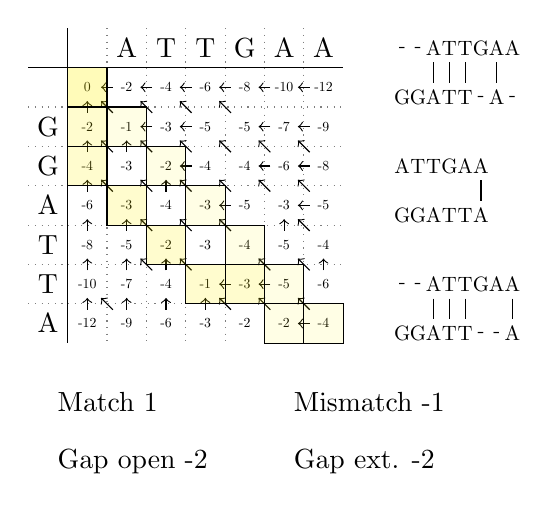
\begin{tikzpicture}[scale=0.5]
    \node [right] at (1,-1) {Match 1};
\node [right] at (7,-1) {Mismatch -1};
\node [right] at (1,-2.5) {Gap open -2};
\node [right] at (7,-2.5) {Gap ext. -2};

\draw [-] (0.5,7.5) -- (8.5,7.5);
\draw [-] (1.5,8.5) -- (1.5,0.5);
\draw [-, dotted, opacity=0.5] (0.5,6.5) -- (8.5,6.5);
\draw [-, dotted, opacity=0.5] (2.5,8.5) -- (2.5,0.5);
	\node at (3,8) {A};
	\draw [-, dotted, opacity=0.5] (3.5,8.5) -- (3.5,0.5);
	\node at (4,8) {T};
	\draw [-, dotted, opacity=0.5] (4.5,8.5) -- (4.5,0.5);
	\node at (5,8) {T};
	\draw [-, dotted, opacity=0.5] (5.5,8.5) -- (5.5,0.5);
	\node at (6,8) {G};
	\draw [-, dotted, opacity=0.5] (6.5,8.5) -- (6.5,0.5);
	\node at (7,8) {A};
	\draw [-, dotted, opacity=0.5] (7.5,8.5) -- (7.5,0.5);
	\node at (8,8) {A};
	\node at (1,6) {G};
	\draw [-, dotted, opacity=0.5] (0.5,5.5) -- (8.5,5.5);
	\node at (1,5) {G};
	\draw [-, dotted, opacity=0.5] (0.5,4.5) -- (8.5,4.5);
	\node at (1,4) {A};
	\draw [-, dotted, opacity=0.5] (0.5,3.5) -- (8.5,3.5);
	\node at (1,3) {T};
	\draw [-, dotted, opacity=0.5] (0.5,2.5) -- (8.5,2.5);
	\node at (1,2) {T};
	\draw [-, dotted, opacity=0.5] (0.5,1.5) -- (8.5,1.5);
	\node at (1,1) {A};

	\node[scale=0.5] at (2,7) {0};
	\node[scale=0.5] at (3,7) {-2};
	\draw [->] (2.65, 6+1) -- (2.35, 6+1);
	\node[scale=0.5] at(4,7) {-4};
	\draw [->] (3.65,6+1) -- (3.35,6+1);
	\node[scale=0.5] at(5,7) {-6};
	\draw [->] (4.65,6+1) -- (4.35,6+1);
	\node[scale=0.5] at(6,7) {-8};
	\draw [->] (5.65,6+1) -- (5.35,6+1);
	\node[scale=0.5] at(7,7) {-10};
	\draw [->] (6.65,6+1) -- (6.35,6+1);
	\node[scale=0.5] at(8,7) {-12};
	\draw [->] (7.65,6+1) -- (7.35,6+1);
	\node[scale=0.5] at (2,6) {-2};
	\draw [->] (2,6 + 0.35) -- (2, 6 + 0.65);
	\node[scale=0.5] at(2,5) {-4};
	\draw [->] (2,6-1 + 0.35) -- (2, 6-1 + 0.65);
	\node[scale=0.5] at(2,4) {-6};
	\draw [->] (2,6-2 + 0.35) -- (2, 6-2 + 0.65);
	\node[scale=0.5] at(2,3) {-8};
	\draw [->] (2,6-3 + 0.35) -- (2, 6-3 + 0.65);
	\node[scale=0.5] at(2,2) {-10};
	\draw [->] (2,6-4 + 0.35) -- (2, 6-4 + 0.65);
	\node[scale=0.5] at(2,1) {-12};
	\draw [->] (2,6-5 + 0.35) -- (2, 6-5 + 0.65);

	\node [scale=0.5] at (3,6) {-1};
	\draw [->] (2.65,6.35) -- (2.35,6.65);
	\node [scale=0.5] at (4,6) {-3};
	\draw [->] (3.65,6.35) -- (3.35,6.65);
	\draw [->] (3.65,6) -- (3.35,6);
	\node [scale=0.5] at (5,6) {-5};
	\draw [->] (4.65,6.35) -- (4.35,6.65);
	\draw [->] (4.65,6) -- (4.35,6);
	\node [scale=0.5] at (6,6) {-5};
	\draw [->] (5.65,6.35) -- (5.35,6.65);
	\node [scale=0.5] at (7,6) {-7};
	\draw [->] (6.65,6) -- (6.35,6);
	\node [scale=0.5] at (8,6) {-9};
	\draw [->] (7.65,6) -- (7.35,6);

	\node [scale=0.5] at (3,5) {-3};
	\draw [->] (2.65,5.35) -- (2.35,5.65);
	\draw [->] (3,5.35) -- (3,5.65);
	\node [scale=0.5] at (4,5) {-2};
	\draw [->] (3.65,5.35) -- (3.35,5.65);
	\node [scale=0.5] at (5,5) {-4};
	\draw [->] (4.65,5.35) -- (4.35,5.65);
	\draw [->] (4.65,5) -- (4.35,5);
	\node [scale=0.5] at (6,5) {-4};
	\draw [->] (5.65,5.35) -- (5.35,5.65);
	\node [scale=0.5] at (7,5) {-6};
	\draw [->] (6.65,5.35) -- (6.35,5.65);
	\draw [->] (6.65,5) -- (6.35,5);
	\node [scale=0.5] at (8,5) {-8};
	\draw [->] (7.65,5.35) -- (7.35,5.65);
	\draw [->] (7.65,5) -- (7.35,5);

	\node [scale=0.5] at (3,4) {-3};
	\draw [->] (2.65,4.35) -- (2.35,4.65);
	\node [scale=0.5] at (4,4) {-4};
	\draw [->] (3.65,4.35) -- (3.35,4.65);
	\draw [->] (4,4.35) -- (4,4.65);
	\node [scale=0.5] at (5,4) {-3};
	\draw [->] (4.65,4.35) -- (4.35,4.65);
	\node [scale=0.5] at (6,4) {-5};
	\draw [->] (5.65,4.35) -- (5.35,4.65);
	\draw [->] (5.65,4) -- (5.35,4);
	\node [scale=0.5] at (7,4) {-3};
	\draw [->] (6.65,4.35) -- (6.35,4.65);
	\node [scale=0.5] at (8,4) {-5};
	\draw [->] (7.65,4.35) -- (7.35,4.65);
	\draw [->] (7.65,4) -- (7.35,4);

	\node [scale=0.5] at (3,3) {-5};
	\draw [->] (3,3.35) -- (3,3.65);
	\node [scale=0.5] at (4,3) {-2};
	\draw [->] (3.65,3.35) -- (3.35,3.65);
	\node [scale=0.5] at (5,3) {-3};
	\draw [->] (4.65,3.35) -- (4.35,3.65);
	\node [scale=0.5] at (6,3) {-4};
	\draw [->] (5.65,3.35) -- (5.35,3.65);
	\node [scale=0.5] at (7,3) {-5};
	\draw [->] (7,3.35) -- (7,3.65);
	\node [scale=0.5] at (8,3) {-4};
	\draw [->] (7.65,3.35) -- (7.35,3.65);

	\node [scale=0.5] at (3,2) {-7};
	\draw [->] (3,2.35) -- (3,2.65);
	\node [scale=0.5] at (4,2) {-4};
	\draw [->] (3.65,2.35) -- (3.35,2.65);
	\draw [->] (4,2.35) -- (4,2.65);
	\node [scale=0.5] at (5,2) {-1};
	\draw [->] (4.65,2.35) -- (4.35,2.65);
	\node [scale=0.5] at (6,2) {-3};
	\draw [->] (5.65,2) -- (5.35,2);
	\node [scale=0.5] at (7,2) {-5};
	\draw [->] (6.65,2.35) -- (6.35,2.65);
	\draw [->] (6.65,2) -- (6.35,2);
	\node [scale=0.5] at (8,2) {-6};
	\draw [->] (7.65,2.35) -- (7.35,2.65);
	\draw [->] (8,2.35) -- (8,2.65);

	\node [scale=0.5] at (3,1) {-9};
	\draw [->] (2.65,1.35) -- (2.35,1.65);
	\draw [->] (3,1.35) -- (3,1.65);
	\node [scale=0.5] at (4,1) {-6};
	\draw [->] (4,1.35) -- (4,1.65);
	\node [scale=0.5] at (5,1) {-3};
	\draw [->] (5,1.35) -- (5,1.65);
	\node [scale=0.5] at (6,1) {-2};
	\draw [->] (5.65,1.35) -- (5.35,1.65);
	\node [scale=0.5] at (7,1) {-2};
	\draw [->] (6.65,1.35) -- (6.35,1.65);
	\node [scale=0.5] at (8,1) {-4};
	\draw [->] (7.65,1.35) -- (7.35,1.65);
	\draw [->] (7.65,1) -- (7.35,1);

\draw [fill=yellow, fill opacity=0.1] (7.5,0.5) rectangle (8.5,1.5);


\draw [fill=yellow, fill opacity=0.1] (6.5,1.5) rectangle (7.5,2.5);


\draw [fill=yellow, fill opacity=0.1] (5.5,2.5) rectangle (6.5,3.5);


\draw [fill=yellow, fill opacity=0.1] (4.5,3.5) rectangle (5.5,4.5);


\draw [fill=yellow, fill opacity=0.1] (3.5,4.5) rectangle (4.5,5.5);


\draw [fill=yellow, fill opacity=0.1] (2.5,5.5) rectangle (3.5,6.5);


\draw [fill=yellow, fill opacity=0.1] (1.5,6.5) rectangle (2.5,7.5);


\draw [fill=yellow, fill opacity=0.1] (5.5,1.5) rectangle (6.5,2.5);


\draw [fill=yellow, fill opacity=0.1] (4.5,1.5) rectangle (5.5,2.5);


\draw [fill=yellow, fill opacity=0.1] (3.5,2.5) rectangle (4.5,3.5);


\draw [fill=yellow, fill opacity=0.1] (2.5,3.5) rectangle (3.5,4.5);


\draw [fill=yellow, fill opacity=0.1] (1.5,4.5) rectangle (2.5,5.5);


\draw [fill=yellow, fill opacity=0.1] (1.5,5.5) rectangle (2.5,6.5);


\draw [fill=yellow, fill opacity=0.1] (1.5,6.5) rectangle (2.5,7.5);


\draw [fill=yellow, fill opacity=0.1] (6.5,0.5) rectangle (7.5,1.5);


\draw [fill=yellow, fill opacity=0.1] (5.5,1.5) rectangle (6.5,2.5);


\draw [fill=yellow, fill opacity=0.1] (4.5,1.5) rectangle (5.5,2.5);

\draw [fill=yellow, fill opacity=0.1] (3.5,2.5) rectangle (4.5,3.5);

\draw [fill=yellow, fill opacity=0.1] (2.5,3.5) rectangle (3.5,4.5);

\draw [fill=yellow, fill opacity=0.1] (1.5,4.5) rectangle (2.5,5.5);

\draw [fill=yellow, fill opacity=0.1] (1.5,5.5) rectangle (2.5,6.5);

\draw [fill=yellow, fill opacity=0.1] (1.5,6.5) rectangle (2.5,7.5);


\node [scale=0.75] (s1) at (10 + 0/2.5, 5) {A};
\node [scale=0.75] (s2) at (10 + 0/2.5, 5-1.25) {G};
\node [scale=0.75] (s1) at (10 + 1/2.5, 5) {T};
\node [scale=0.75] (s2) at (10 + 1/2.5, 5-1.25) {G};
\node [scale=0.75] (s1) at (10 + 2/2.5, 5) {T};
\node [scale=0.75] (s2) at (10 + 2/2.5, 5-1.25) {A};
\node [scale=0.75] (s1) at (10 + 3/2.5, 5) {G};
\node [scale=0.75] (s2) at (10 + 3/2.5, 5-1.25) {T};
\node [scale=0.75] (s1) at (10 + 4/2.5, 5) {A};
\node [scale=0.75] (s2) at (10 + 4/2.5, 5-1.25) {T};
\node [scale=0.75] (s1) at (10 + 5/2.5, 5) {A};
\node [scale=0.75] (s2) at (10 + 5/2.5, 5-1.25) {A};
\draw [-] (s1) -- (s2);
\node [scale=0.75] (s1) at (10 + 0/2.5, 2) {-};
\node [scale=0.75] (s2) at (10 + 0/2.5, 2-1.25) {G};
\node [scale=0.75] (s1) at (10 + 1/2.5, 2) {-};
\node [scale=0.75] (s2) at (10 + 1/2.5, 2-1.25) {G};
\node [scale=0.75] (s1) at (10 + 2/2.5, 2) {A};
\node [scale=0.75] (s2) at (10 + 2/2.5, 2-1.25) {A};
\draw [-] (s1) -- (s2);
\node [scale=0.75] (s1) at (10 + 3/2.5, 2) {T};
\node [scale=0.75] (s2) at (10 + 3/2.5, 2-1.25) {T};
\draw [-] (s1) -- (s2);
\node [scale=0.75] (s1) at (10 + 4/2.5, 2) {T};
\node [scale=0.75] (s2) at (10 + 4/2.5, 2-1.25) {T};
\draw [-] (s1) -- (s2);
\node [scale=0.75] (s1) at (10 + 5/2.5, 2) {G};
\node [scale=0.75] (s2) at (10 + 5/2.5, 2-1.25) {-};
\node [scale=0.75] (s1) at (10 + 6/2.5, 2) {A};
\node [scale=0.75] (s2) at (10 + 6/2.5, 2-1.25) {-};
\node [scale=0.75] (s1) at (10 + 7/2.5, 2) {A};
\node [scale=0.75] (s2) at (10 + 7/2.5, 2-1.25) {A};
\draw [-] (s1) -- (s2);
\node [scale=0.75] (s1) at (10 + 0/2.5, 8) {-};
\node [scale=0.75] (s2) at (10 + 0/2.5, 8-1.25) {G};
\node [scale=0.75] (s1) at (10 + 1/2.5, 8) {-};
\node [scale=0.75] (s2) at (10 + 1/2.5, 8-1.25) {G};
\node [scale=0.75] (s1) at (10 + 2/2.5, 8) {A};
\node [scale=0.75] (s2) at (10 + 2/2.5, 8-1.25) {A};
\draw [-] (s1) -- (s2);
\node [scale=0.75] (s1) at (10 + 3/2.5, 8) {T};
\node [scale=0.75] (s2) at (10 + 3/2.5, 8-1.25) {T};
\draw [-] (s1) -- (s2);
\node [scale=0.75] (s1) at (10 + 4/2.5, 8) {T};
\node [scale=0.75] (s2) at (10 + 4/2.5, 8-1.25) {T};
\draw [-] (s1) -- (s2);
\node [scale=0.75] (s1) at (10 + 5/2.5, 8) {G};
\node [scale=0.75] (s2) at (10 + 5/2.5, 8-1.25) {-};
\node [scale=0.75] (s1) at (10 + 6/2.5, 8) {A};
\node [scale=0.75] (s2) at (10 + 6/2.5, 8-1.25) {A};
\draw [-] (s1) -- (s2);
\node [scale=0.75] (s1) at (10 + 7/2.5, 8) {A};
\node [scale=0.75] (s2) at (10 + 7/2.5, 8-1.25) {-};


  \end{tikzpicture}
  \caption{Score, routing table and the extracted alignments}
  \label{traceBack2}
  \end{subfigure}
%% font sizes available in latex
%% tiny, scriptsize, footnotesize, small, normalsize, large
%% Large, LARGE, huge, Huge
%%\begin{figure}[ht]
  \begin{subfigure}{0.5\textwidth}
  \begin{tikzpicture}[scale=0.3]
%    \draw [help lines, opacity=0.5] (0,0) grid (22,12);
%    \foreach \x in {1,2,...,19} \node [font=\small] at (\x,0) {\x};
%    \foreach \y in {1,2,...,12} \node [font=\small] at (20,\y) {\y};
    %% the diameter of the circle can be set with minimum width
    \node (s1) [rectangle, scale=0.8] at (13,3) {1};
    \node (s2) [rectangle, scale=0.8] at (11,5) {2};    
    \node (s3) [rectangle, scale=0.8] at (9,7) {3};
    \node (s4) [rectangle, scale=0.8] at (7,9) {4};
    \node (s5) [rectangle, scale=0.8] at (5,11) {5};
    \node (s6) [rectangle, scale=0.8] at (3,13) {6};

    \node (s7) [rectangle, scale=0.8] at (9,5) {7};
    \node (s8) [rectangle, scale=0.8] at (7,5) {8};
    \node (s9) [rectangle, scale=0.8] at (5,7) {9};
    \node (s10) [rectangle, scale=0.8] at (3,9) {10};
    \node (s11) [rectangle, scale=0.8] at (1,11) {11};
    \node (s12) [rectangle, scale=0.8] at (1,13) {12};

%    \node (s13) [rectangle, scale=0.8] at (11,3) {13};   

    \draw [->] (s1) -- (s2);
    \draw [->] (s2) -- (s3);
    \draw [->] (s3) -- (s4);
    \draw [->] (s4) to (s5);
    \draw [->] (s5) to (s6);
    
    \draw [->] (s2) to (s7);
    \draw [->] (s7) to (s8);
    \draw [->] (s8) to (s9);
    \draw [->] (s9) to (s10);
    \draw [->] (s10) to (s11);
    \draw [->] (s11) to (s12);

%    \draw [->] (s1) to (s13);
%    \draw [->] (s13) -- (s7);

    %% redraw it, but offset to the right
    \node (s1) [rectangle, scale=0.8, opacity=0.4] at (20,3) {1};
    \node (s2) [rectangle, scale=0.8, opacity=0.4] at (18,5) {2};    
    \node (s3) [rectangle, scale=0.8, opacity=0.4] at (16,7) {3};
    \node (s4) [rectangle, scale=0.8, opacity=0.4] at (14,9) {4};
    \node (s5) [rectangle, scale=0.8, opacity=0.4] at (12,11) {5};
    \node (s6) [rectangle, scale=0.8, opacity=0.4] at (10,13) {6};

    \node (s7) [rectangle, scale=0.8] at (16,5) {14};
    \node (s8) [rectangle, scale=0.8] at (14,5) {15};
    \node (s9) [rectangle, scale=0.8] at (12,7) {16};
    \node (s10) [rectangle, scale=0.8] at (10,9) {17};
    \node (s11) [rectangle, scale=0.8] at (8,11) {18};
    \node (s12) [rectangle, scale=0.8] at (8,13) {19};

    \node (s13) [rectangle, scale=0.8] at (18,3) {13};   

 %   \draw [->] (s1) -- (s2);
 %   \draw [->] (s2) -- (s3);
 %   \draw [->] (s3) -- (s4);
 %   \draw [->] (s4) to (s5);
 %   \draw [->] (s5) to (s6);
    
%    \draw [->] (s2) to (s7);
    \draw [->] (s7) to (s8);
    \draw [->] (s8) to (s9);
    \draw [->] (s9) to (s10);
    \draw [->] (s10) to (s11);
    \draw [->] (s11) to (s12);

    \draw [->] (s1) to (s13);
    \draw [->] (s13) -- (s7);

    \draw [-, opacity=0] (1, -4) -- (4, -4);
    \draw [-, opacity=0] (1, 15.16) -- (4, 15.16); 

  \end{tikzpicture}
  \caption{The recursive tracing order. Left: the two
  first alignments; right: the final alignment}
  \label{recurseOrder}
  \end{subfigure}
  \caption{Recursive extraction of the alignments from the route table. The order in
  which the routes are followed are indicated in (b). The first alignment
  is extracted by following the diagonal routes from the bottom left corner (1-6). The
  second alignment is then started by following the pointer at the last branch point
  encountered during the first extraction (2). Finally we start at the first branch point
  at position 1 and follow the last route (13-19). Note that the order of the alignments in (b)
  does not correspond to this order.}
  \label{alExtraction}
\end{figure}
To demonstrate the process, consider Fig. \ref{alExtraction}. We start from the lower
right corner. In the first cell we find two arrows (diagonal and left; i.e. a route
encoding of 3). This means that \verb|$routes[$i][$j] & 1| is TRUE (as it returns a non-0
value); we then increment the \verb|$route_count| variable and prepend the aligned sequences
(stored in \verb|$a_al[$n]| and \verb|$b_al[$n]|). Finally we call the \verb|obtain_alignment|
function with decremented values of \verb|$i| and \verb|$j|. When this happens we will
enter a new function, and any variables declared within the function will be reset (eg. \verb|$route_count|
is now 0 again). Here we do exactly the same thing, and as we again have a diagonal route
we follow that, calling \verb|obtain_alignment| recursively until \verb|$i| and \verb|$j| are 0 or
we do not have any more links to follow. All these subsequenct calls to \verb|obtain_alignment|
have to return before the first instance of the function can proceed to the second step (i.e. 
\verb|if($routes[$i][$j] & 2)|). This means that the first branch point encountered
(in this case in the first cell examined) will be the last one to be followed. More generally,
the first instance of the function called will be the last one to complete.

At the first step of the extraction process we looked at the bottom right cell. This has
two arrows (and a routing value of 3) and we first incremented \verb|$route_count| and then
called \verb|obtain_alignment| with \verb|$i-1| and \verb|$j-1|. That call returns only
after all subsequent recursive calls to \verb|obtain_alignment| have completed (which in this
case means after having extracted two complete alignments). When that call returns, the funtion
goes to the next step:

\begin{minted}[fontsize=\scriptsize,bgcolor=lightgray,linenos]{perl}
  if($routes[$i][$j] & 2){
    # if $route_count is larger than 0, we have already completed
    # at least one alignment and we need space for one more, so
    # we push @a_al and @b_al, adding the alignments obtained before
    # getting here.
    # ($al, and $bl were defined as local variables at the beginning 
    # of the function)
    if($route_count > 0){  
      push @a_al, $al;
      push @b_al, $bl;
    }
    ## we define the local variable $an as the current last index of
    ## of @a_al. This is the alignment string that will be modified
    ## here and in recursive calls to the function.
    my $an = $#a_al;
    $route_count++;
    $a_al[$an] = "-".$a_al[$an];
    $b_al[$an] = $b[$j-1].$b_al[$an];
    obtain_alignment($i, $j-1, $an); 
  }
\end{minted}
 
We first have to check whether or not we have already called and returned from
\verb|obtain_alignment|. If this is the case we have already obtained at least
one alignment, and we need to start a new one. To do this, we extend the \verb|@a_al| and
\verb|@b_al| arrays (using \verb|push|) with the sequences that had been aligned when this
function was first entered (\verb|$al| and \verb|$bl|).
Since we are moving leftwards in the table, we then prepend \verb|$a_al[$an]| and \verb|$b_al[$an]|
with '-' or a character from the top sequence respectively. Finally we call 
\verb|obtain_alignment| with the coordinates corresponding with the cell to the left.

This can be a little bit confusing, and is rather difficult to explain clearly. To understand
it you probably have to spend some time to think about it. I will not require you to understand
recursion, but I may include an optional question on the exam on the topic as it is a much
used technique.

\subsection{Additional stuff}
\label{sec-1-4}
As mentioned above, I also wrote a non-recursive form of the extraction (step3b). 
I'll leave it to you to work that function out yourself. It does not contain
anything strange that's not already been explained above. For this script I also added
a small function that prints out the alignment in a somewhat prettier manner.

I also modified this last script to allow it to use affine gap penalties (i.e. different
penalties for gap insertions and extensions): \verb|needleman_wunsch_step4b.pl|. 
The number of changes are rather small
and it should not be difficult to understand. However, because the final routing table
can give rise to non-optimal alignments I also added a function that calculates the scores
for the extracted alignments. This can be used to select only those that give a maximal
score. I also added a small modification to the \verb|print_alignment| function.

\end{document}



